\documentclass[12pt]{article}
\usepackage{amsmath}
\usepackage{ amssymb}
\usepackage{amsthm}
\usepackage{fancyhdr}
\usepackage{hyperref}
\usepackage{xcolor}
\usepackage{minted}
\usepackage{listings}
\usepackage{graphicx}
\usepackage[numbers]{natbib}
%\graphicspath{ {./} }
\usemintedstyle{pastie}

\definecolor{codegreen}{rgb}{0,0.6,0}
\definecolor{codegray}{rgb}{0.5,0.5,0.5}
\definecolor{codepurple}{rgb}{0.58,0,0.82}
\definecolor{codebg}{rgb}{0.95,0.95,0.92}
\lstdefinestyle{mystyle}{ backgroundcolor=\color{codebg}, commentstyle=\color{codegreen}, keywordstyle=\color{magenta}, numberstyle=\tiny\color{codegray}, stringstyle=\color{codepurple}, basicstyle=\ttfamily\footnotesize, breakatwhitespace=false, breaklines=true,  captionpos=b,  keepspaces=true,  numbers=left,  numbersep=5pt,  showspaces=false,  showstringspaces=false, showtabs=false,  tabsize=2
}
\lstset{style=mystyle}

\title{title}
\author {Alex Oswald}

\setlength{\headheight}{28pt}
\pagestyle{fancy}
\fancyhf{}
\fancyhead[L]{Alex Oswald}
\fancyhead[C]{EECE 4991 Report}
\fancyhead[R]{Summer 2023}
\fancyfoot[C]{\thepage}


\begin{document}
% fix for images?
%\shorthandoff{=}
 
\begin{center}\Large Exploration \& Modeling of Micro- and Mesa-Scale Small-Loop Antennae \end{center}

\begin{section} {Near-Field Probes: Fundamentals}

\subsection{Types \& Applications}

The reactive near-field of electromagnetism is defined as the region close to a radiating source where the electric and magnetic fields are strongly coupled and do not propagate as plane waves. Near-field electromagnetic interactions are distinctly reactive and tend have rapid changes in field strength over short distances from their source. The near-field operates within the immediate vicinity of a source, typically within a wavelength, whose distance is characterized by $r$ in the equation below. The principal of this range is such that the electric and magnetic fields do not independently propagate energy, rather, they emanate from various electromagnetic sources and interact with others. Commonly, this is referred to as electromagnetic interference (EMI) radiating from electronics. The two primary components of the near-field are the electric-field (E-Field) and the magnetic-field (B-Field). The E-Field arises from stationary charges and is responsible for interactions due to electric charge differences. In contrast, the B-Field is generated by moving charges, typically current flow, and accounts for magnetic effects in the immediate environment of the source \cite{kanda_standard_1993}.

\[
r = \sqrt{ \frac{\lambda}{2 \pi} }
\]

In the realm of electromagnetic compatibility and diagnostics, Near-Field Probes (NFPs) have established themselves as indispensable tools. Predominantly, NFPs are classified based on their capacity to detect either E-Field or B-Field interactions. H-Field (Magnetic) probes, principally the Electrically-Small Loop and Magnetic Monopole probes, specialize in sensing magnetic disturbances in the environment. Next, the E-Field (Electric) probes, such as the Open-ended Coaxial and Dipole probes, are adept at identifying electric field variances. The third type is the Hybrid Near-Field Probe, that attempts to combine each field strength using combination probes, like the Biconical or Bilog Antennae, which harness the capability to sense both electric and magnetic fields simultaneously \cite{dyson_characteristics_1965}. Each type of probe has its distinct applications, bandwidth, and design, making them suited to specific tasks within electromagnetic studies \cite{huang_antennas_2021}.

Briefly touching upon some other probes: The Magnetic Monopole probes, similar in magnetic field detection to the small-loop antenna, have a narrower focus but offer precise point measurements and are not passive \cite{kanda_standard_1994}. Open-ended Coaxial and Dipole probes cater to E-Field detections, with the former being popular in localized EMI studies due to its broadband nature and the latter showing merit in applications like antenna pattern measurements. The Log-Periodic Probe, using its unique log-periodic antenna design, is unparalleled in spectrum analysis and captures a wide frequency bandwidth, making it particularly useful in broadband EMI analysis. The Biconical Probe, utilizing its dual conical elements, can detect both E-Fields and B-Fields. It shines in broadband measurements and is a staple in EMI chambers \cite{dyson_characteristics_1965}. Lastly, the Active Amplifier Probe, a field-agnostic augmentation to a probe, augments sensitivity by integrating an active amplifier, making it invaluable in scenarios demanding high precision and reduced extraneous pickups, and often a necessity for signal reception in all manner of passive probes \cite{huang_antennas_2021}.

\subsection{Magnetic Near-Field Probes}

This investigation will principally focus on the Electrically Small-Loop Antenna. The electrically small loop, as its name suggests, has a size much smaller than the wavelength it is intended to measure, typically characterized by a circumference less than one-tenth of the wavelength. This nature offers several key advantages: compactness, enhanced spatial resolution, and minimized interference from surrounding fields. It primarily is only sensitive to magnetic fields, which makes it a specialized tool making it especially adept at identifying and localizing sources of active current or electromagnetic interference (EMI). Further, this antenna's applications are wide-ranging; its prominence in pinpointing current leakage paths and magnetic interference in PCB boards and other intricate electronics.

Yet, prior to continuation, an additional type of sensor to reactive magnetic fields is the Hall-Effect Sensor. It is similar to the small-loop and magnetic monopole antennas in it's B-Field specific measurements, but they different vastly in many other aspects of design.  The Hall-Effect sensor is based on the Hall effect principle, where a voltage difference is generated across a conductor when exposed to a magnetic field perpendicular to the direction of current flow. Hall sensors typically only have dimensions on the order of millimeters. Unlike the Small-Loop and Magnetic Monopole antennas, the Hall-Effect sensor is primarily geared towards detecting static, DC, and slowly varying magnetic fields, making it highly applicable in low-frequency scenarios such as current measurement and position sensing. It's smaller size also owes to pinpointing EMI with great precision, owing to it's employment as a physical verification measure in the silicon wafer industry. Its functionality is rooted in its unique ability to measure the magnitude and direction of the magnetic field, making it especially valuable in applications such as position sensing, rotational speed detection, and direct current measurements \cite{shede_leakage_2017}.

In summary, while all the aforementioned probes offer specific advantages based on their design and application domains, the Electrically Small-Loop Antenna stands out for its versatility, precision, and aptness for magnetic field studies in EMC. With new technologies regarding the 3D printing of MEMs devices, the small-loop antenna is ripe for miniaturization and optimization for new spectra.

\end{section}
\begin{section} {Small-Loop Antennae}

\subsection{The Circular Small-Loop}

\subsubsection{Design and Usage}

In review, electrically small-loop antennas, commonly referred to as magnetic loops or tuned loops, are a type of passive, resonant antenna most used as receiving antennae. Small-loop antennae are generally $ \frac{1}{3} - \frac{1}{100} $ the size of the target wavelength. They may take the shape of any closed loop, but the optimal form is a circular loop as they are the most efficient at capturing the field strength perpendicular to the plane of the coil in accordance with Ampére's law. The small-loop is effected by both the electric and magnetic components of an electromagnetic field, but is most-reactive to the magnetic component, or the B–field. Thus, when employed in high-frequency applications they are most often used as electromagnetic interference (EMI), while historically, their application has been in near-field communications, radio-frequency identification (RFID), and magnetic resonance imaging (MRI) \cite{kanda_standard_1993}.

The primary parameter of interest for small-loop antennas is their radiation resistance, which is a measure of their efficiency. Inherently, small-loop antennas have a low radiation resistance, which results in low efficiency. However, the radiation resistance can be increased by increasing the area or the number of turns of the loop. Moreover, small-loop antennas exhibit a high quality factor (Q), which leads to a narrow bandwidth. This bandwidth can be broadened by introducing a loading resistance.

\subsubsection{Resonance and Response}

The induced voltage \(V_i\) in an electrically-small loop antenna is related to its frequency, the number of turns, and its area. To obtain a flat frequency response, the quality score, $Q$, of the antenna should be reduced using a loading resistance. The resonance of the antenna arises due to the distributed capacitance of the loop, the gap capacitance, and the input capacitance of an attached amplifier. This resonates with the inductance of the loop, as depicted in an equivalent circuit \cite{kanda_standard_1993}. This gives rise to the antenna's response as:

\[
\frac{V_0}{V_i} = \frac{-j \frac{1}{\delta}}{\frac{1}{Q} + j \left( \frac{1}{\delta} - \delta \right)}
\]

Where the constituent parts including $Q$ and $\delta$ can be defined by the loading resistance, $R$, input angular frequency $\omega$, resonant angular frequency $\omega_0$, capacitance $C$, and inductance $L$ comprise:

\begin{align*}
Q = \frac{R}{\omega_0 L} = \omega_0 R C,
\qquad
\delta = \frac{\omega}{\omega_0},
\qquad
\omega_0 = \frac{1}{\sqrt{LC}}.
\end{align*}

\subsubsection{Inductance and Capacitance of the Loop}

The inductance and self-inductance of a small-loop antenna depend on the loop shape and, in the case of a circular small-loop, the number of turns in the loop.  This inductance represents the loop's ability to oppose changes in current, manifested as stored magnetic energy, which results in a voltage opposing the change of the current in the loop. As the number of turns, $ N $, in the loop increases, the inductance rises proportionally to $ N^2 $. This parameter significantly impacts the reactive component of the antenna impedance, the resonant frequency $ f_0 $, and determines its lower frequency limit, and influences the resonant frequency. An increase in inductance will lead to a decrease in the resonant frequency.

The high-order approximation of the low-frequency inductance of a single-turn loop, where $\mu$ is the permeability of the medium, is given by:

\[
L = \mu b \left[ \ln\left(\frac{8b}{a}\right) - 2 \right],
\]

and in an $N$-turn loop, the inductance is $N^2$ times that of a single-turn loop. Though, generally as the radius of the loop, $b$, is much greater than the radius of the wire, $a$, or $ b \gg a $, one can represent the inductance as (where $ N^2=(1)^2 $ for a single-turn loop):

\[
L \approx N^2 \times \mu b \ln \left( \frac{b}{a} \right).
\]

Conversely, the loop's self-capacitance arises from potential difference in the electric field across the loop, or between each adjacent turn in the coil, reflecting the stored electric energy in the field across the loop. This capacitance significantly impacts the antenna's reactive impedance component and affects its higher frequency limit. With a higher self-capacitance value one can expect a lower resonant frequency, though adding more loops will not linearly increase the capacitance \cite{whiteside_loop_1964}. The mid-order approximation of the capacitance in a single-turn, circular small-loop is described:

\[
C = \frac{2 \epsilon_r b}{\ln\left(\frac{8b}{a}\right) - 2},
\]

where $\epsilon$ is the permittivity of the loop medium; defined as $ \epsilon = \epsilon_r \times \epsilon_0 $ where $\epsilon_r$ is the relative permittivity of the medium (often a dielectric constant), and $\epsilon_0$ is the permittivity of free space \cite{huang_antennas_2021}. Since the relationship of the loop and wire radii is typically such that $ln(b/a) > 1$, this can be approximated as:

\[
C \approx \frac{2 \epsilon b}{\ln \left( \frac{b}{a}\right)}.
\]

The transfer function of an electrically small loop antenna is given,

\[
T(f) = \frac{V_0}{V_i} = \omega_0 \mu N S \left| \frac{1}{Q} + j \left( \delta - \frac{1}{\delta} \right) \right|^{-1},
\]

and the normalized transfer function is discovered as:

\[
T_n(f) = \left| \frac{1}{Q} + j \left( \delta - \frac{1}{\delta} \right) \right|^{-1}.
\]

\subsubsection{Conclusion}

Small-loop antennas offer a compact solution for many frequency applications, especially when size constraints are critical. However, the inherent characteristics like the high Q, large bandwidth, and low radiation resistance necessitate careful design considerations . By understanding the key design equations and characteristics, one can optimize these antennas for various applications.

\subsection{Alternative Closed-Loop Antenna Designs}

One of the most important design considerations of the circular small-loop antenna is that it is single-directional.. It reacts to the magnetic field circulating perpendicular to the plane parallel to the loop. This makes it poised for great field-vector measurements, but also limits its effectiveness in isotropic field measurements, or a field measurement invariant with respect to direction. This specific constraint, is where other shapes unlike the circle may

In addition to the circular small-loop antenna, several other geometries have emerged to serve particular applications and address specific challenges in the realm of electromagnetic studies.  Most common is the square loop antenna alternative design.  In addition, there are the helical loop antennae that include extra parameters such as pitch, loop gap, and the number of turns.  Following, is the ferrite-loop that contains a magnetically permeable core (e.g. an iron rod) through it's center which can significantly increase the magnetic response of the still-passive loop. Finally, there are more exotic and, often, application-specific small-loops under active development in 3D forms that optimize for isotropic resonance of the loop antenna.

The square loop, frequently observed in amateur radio configurations, is predominantly utilized for lower resonant frequencies, necessitating larger loops. The most common form was once the "quad" antenna including two separated paralell loops with a parasitic wire strapped in a 'x' across each loop to add a parasitic element. However, the square doesn't add many benefits and merely facilitates a mildly sub-optimal radiation resistance. Yet, the inclusion of squares in the design of 3D small-loop antennae is common practice to increase manufacturability.

\subsubsection{The Helical Antenna}

The Helical Antenna offers a slightly different variation. While it can be perceived as an offshoot of the dipole or monopole antenna, its resemblance and behavior also align closely with loop antennas. When examining the helix in its \textit{Normal Mode}, a condition where both the diameter of the helix (D) and its total length are substantially smaller than the wavelength (\(D \ll \lambda\)), it demonstrates characteristics akin to a broadside radiation pattern. Conversely, its \textit{Axial Mode} becomes less pertinent when the circumference of the helix approximates the wavelength, but this would not be applicable in the small-loop design (\(C = \pi D \approx \lambda\)). A notable aspect of the helical antenna is its narrow bandwidth, stemming from its input impedance's heightened sensitivity to frequency changes. When employed alongside a ground plane, its radiation mimics that of a monopole, predominantly exhibiting vertical polarization. Its radiation resistance can be approximated simply when in its dipole formation, but requires simulation to divine when contextualized in the self-grounded small-loop design  \cite{huang_antennas_2021}. The helix is not typically considered in the context of a closed small-loop as the design requires re-traversing the length of the helix, but the helix is an inefficient radiator and could substantially build on the circular small-loop design. This considered, what makes the helical small-loop antenna difficult to produce and design is the innate self-capacitance between successive loops that limit their modelling to high-compute FDTD electromagnetic simulations.

\subsubsection{Ferrite Antennas}

Ferrite loading an antenna offers a promising avenue to enhance the performance of electrically small loop antennas. Principally, it works to amplifying the signal-to-noise ratio for a loop antennas. As considered in Section 2.1.3, the magnetic permeability of an antenna's metal is directly proportional to it's inductance which is in an inverse relationship with the capacitance controlling the quality factor; in other words, by adding the magnetically permeable ferrite core one can drastically change the design parameters of the small-loop antenna and allow for a more effective miniaturization of an otherwise unaltered design (e.g. circular small loop, helix, or 3D isotropic). The derived formulas, rooted in the reaction concept, provide insights into the antenna's impedance, efficiency, and Q-factor when ferrite-loaded, with distinctions based on the internal magnetic field and the ferrite's shape, like ellipsoidal or rod-shaped cores. This nuanced approach, taking into account the size and shape of the ferrite core, highlights the complexities and potential gains in adapting ferrite-loaded designs \cite{rumsey_electrically_1956}.

Before the advent of modern simulation techniques, a formulaic approximation was derived by Rumsey and Weeks to find the reactive resistance for a ferrite loaded loop antenna in a given an incident magnetic field  $H_0$ and it's component normal to the loop $H_C$, free space wavelength $\lambda$, loop area $A$, and relative permeability $k = \mu / \mu_0 $ (discounting the complex aspect) \cite{rumsey_electrically_1956}:

\[
R_R = \frac{31171}{\lambda^{4}} \left| \iint_{A} \frac{k H_C}{H_O} \delta A \right|^{2} .
\] 

\subsubsection{Isotropic \& 3-D Antennas}

Considering more contemporary research, 3D antennas have garnered considerable attention for their novel potential to amplify the dimensionality across countless domains in microelectronic manufacturing, of which isometric resonant small-loop antenna configurations are not immune.

Jin and Ali, for instance, proposed a groundbreaking 3D cubic loop antenna characterized by an almost isotropic pattern. Specifically tailored for RFID measurements operating around 1 GHz, their design showcased the versatility of 3D geometries in achieving balanced field patterns \cite{jin_novel_2014}.

Rajaram, on a similar trajectory, introduced a compact, open-ended multiband loop antenna tailored for 4G mobile phone applications. Uniquely, his design featured two concentric loops separated by a distance akin the loop radius. They were able to optimize their 3D model to a very consistent but slightly lossy coplanar and cross-planar radiation patterns; in evaluation of where their antenna and radiation efficiencies coupled most on a plot of loss percentage over a frequency band, they selected the bandwidths of 0.8 GHz, 1.8 GHz, and 2.4 GHz as suitable bandwidths for their design \cite{rajaram_compact_2015}.

Sivaraman, adopting a divergent approach in 2017, integrated three distinct loops, each positioned on a perpendicular face of a cube. Through measuring the reactance of each component, he deduced an isotropic outcome. Despite its compactness—around 2 mm—this design did compromise on spatial accuracy, underscoring the intricate balance between form factor and performance \cite{sivaraman_three_2017}. Further contributing to the burgeoning field of 3D antenna design, a study in 2015 illustrated the design of an isotropic 3D antenna tailored for 24 GHz ISM band applications, further validating the expansive possibilities within the realm of 3D small-loop antenna configurations \cite{sravani_design_2015}.

In temporary conclusion, after considering these attempts of designing 3D isometric small-loop antennas, many incurred common themes and pitfalls. While the simulations varied in rigor and somewhat in methodology, nearly all of them faced discrepancies in frequency shifts and loss patterns between the simulated and measured quantities. This serves to emphasize a continued passion for iterating and prototyping without over-reliance on EM Sim. modelling, and simultaneously developing better simulation techniques.

\end{section}

\begin{section} {Additive Manufacturing of 3D Electronics}

\subsection{State of the Industry and Projections}

The rise of additive manufacturing on the mesa-, micro-, and nano-scales continues to make a profound impact on the hardware, compute, and the component design process itself. With an era of fast-prototyping encroaching, chips scaling to chiplets, and the ability to construct intricate micro- and nano-electromechanical sensors from a single print process, a transformative shift in electronic component design and manufacturing is underway.

Rapid prototyping has led to an accelerated pace of discovery in novel and unique electrical engineering (EE) component designs. At the heart of these advancements are a new generation of AME, multi-material printers. By enabling faster prototyping in the lab, the cascade of benefits permeates the entire electronic sector, optimizing everything from material consumption to design flexibility \cite{divakaran_comprehensive_2022}.

Building upon this paradigm shift, Inkjet Printing (IJP) emerges as a pivotal additive manufacturing tool. Rooted in the pioneering efforts of Brother Industries and Texas Instruments, IJP meticulously crafts 3D structures via a layer-by-layer deposition method \cite{divakaran_comprehensive_2022}. By employing a drop-on-demand mechanism, ink droplets are precisely placed on a powder bed, mirroring the blueprints of 3D CAD imagery. Such accuracy, governed by fluid physics principles, ensures meticulous binder-powder interactions that are pivotal for the seamless integration of components.

Not far behind is Aerosol Jet Printing (AJP), a groundbreaking contactless direct write technique, introduced by OPTOMEC Inc. Renowned for its precision, AJP seamlessly integrates with a spectrum of electronic applications, attributed largely to its streamlined processability. The precision and resolution delivered by AJP earmark it as an ideal solution for micro-mechanical and micro-optical devices \cite{ponis_systematic_2021}.

Projecting forward, the narrative of the electronics sector appears intrinsically linked to 3DP methods like IJP and AJP. As demands pivot towards intricate, efficient, and miniaturized solutions, these additive manufacturing strategies will inevitably become cornerstones. Embracing 3DP for electronics transcends mere futuristic vision; it's the defining trajectory of the present. As we tread this path, a new epoch of portable electronics emerges, hallmarked by unparalleled energy storage and a sophisticated interconnected landscape, thus underscoring the imperative of persistent exploration and innovation. 

\subsection{Nano-Dimension Dragonfly IV}

Within this revolution, Nano Dimension is noteworthy for their contributions in providing a printer that upgrades the very way we can design.  Moving on from a 2D, layer by layer, always the same plane, design strategy their new printers offer Plated Through Hole Vias, Blind and Buried Vias, Staggered and Skip Vias, and Stacked Vias.

This advancement allows designers to circumventing design limitations inherent to conventional PCBs by allowing for direct z-axis connections where traditional PCBs required some more maneuvering and planning in a 2D, though layered, plane.
The 3-dimensional trace increases routing density on it's own, but even allots for the capacity to specify and vary the thickness of a segment through a 3D-trace. And instead of venturing to meta-materials, they simplified and expanded by offering multi-materials \cite{__2022}.

Furthermore, AME adeptly tackles power distribution challenges like the IR drop, by dynamically adjusting the power layer's thickness in tandem with current density variations. The design flexibility extends to intricate geometries, integrated 3D components, and avant-garde packaging solutions, all the while yielding a reduced component count, compact form factors, and enhanced overall performance.

\end{section}

\begin{section} {NFP Design and Simulation}

Building upon the design equations delineated in Section 2.1 and taking into account the associated design constraints, we constructed a Jupyter Notebook tailored to scrutinize an extensive dataset encompassing 2.4 million rows of parameters for circular small-loop antennas. To ensure the accuracy and reliability of these equations, they were subsequently validated through the MATLAB symbolic math toolbox, as illustrated in the subsequent sections.

To start, the design equations were verified and simplified using the MATLAB symbolic math toolbox as demonstrated below.

\begin{minted}{matlab}
>> syms Q R X0 w0 L C mu epsilon a b
>> eqQ = Q == R / X0;
>> eqX0 = X0 == w0 * L == 1 / (w0 * C);
>> eqw0 = w0 == 1 / sqrt(L * C);
>> eqL = L == mu * b * (log(8*b/a) - 2);
>> eqC = C == (2 * epsilon * b) / (log(8*b/a) - 2);
>> subs(subs(subs(subs(eqQ, X0, eqX0), w0, eqw0), L, eqL), C, eqC)

ans = Q == (R*(C*L)^(1/2))/L 
 == (2*R*b*epsilon)/((log((8*b)/a) - 2)*(2*b^2*epsilon*mu)^(1/2))

>> subs(subs(subs(subs(eqQ, X0, eqX0), w0, eqw0), C, eqC), L, eqL)

ans = Q == (R*(C*L)^(1/2))/L 
 == (2*R*b*epsilon)/((log((8*b)/a) - 2)*(2*b^2*epsilon*mu)^(1/2))
\end{minted}

Following, a python Jupyter notebook was created for data analysis and mass-simulation capacity, at step and within the parameters defined by the limits of the NanoDimension Dragonfly IV printer. The functions for calculation and methodology can be found in Appendix A attached. Included in the code snippet below are the parameters employed for testing the circular small-loop antennae at scale.  For wire radius $a$ and loop radius $b$, the minimum, maximum, and step values are provided in meters.

\begin{minted}{python}
df = gen_data(eps=eps_0,  mu=mu_0,  R=50,
               a=(17e-6,  3.0e-3,   5e-6),
               b=(50e-6,  40.0e-3,  10e-6),
               N=None,    rN=None )
df = add_z_order(df, 'a', 'b')
df = normalize_df(df)
\end{minted}

After adding a dimensionality-reduction measure according to the Z-Order Curve based on the Morton Order, the following plots were constructed to review.

\begin{figure}
    \centering
    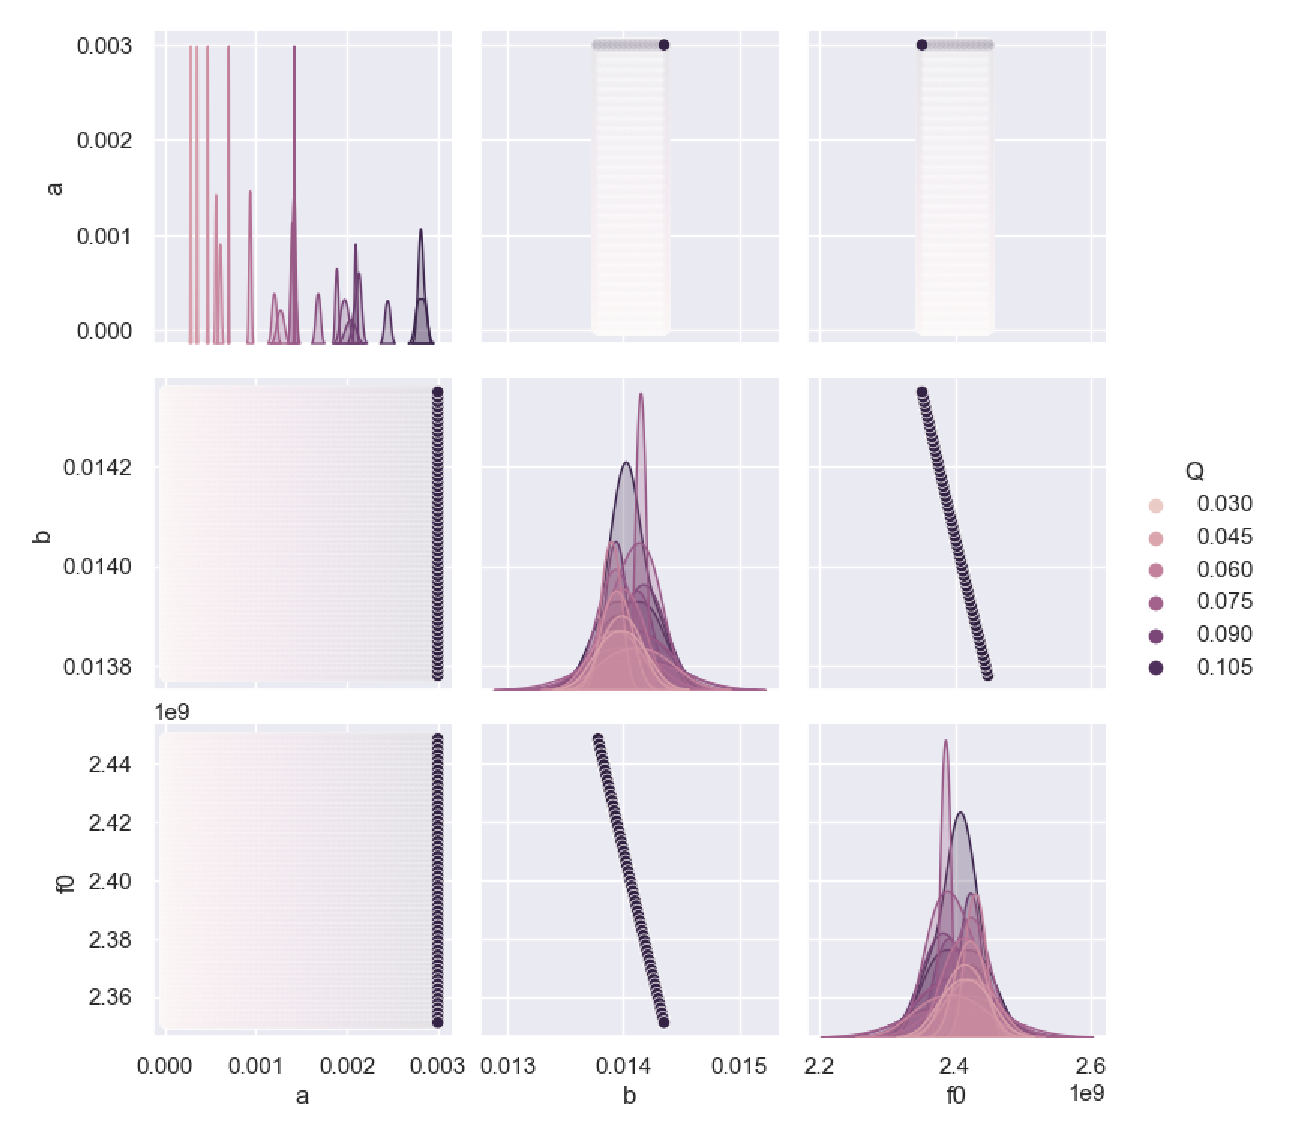
\includegraphics[scale=0.30]{images/plot_abQf0.eps}
    \caption{Figure 1: A seaborn pairplot of the wire radius (a), loop radius (b), and the resonant frequency.  The diagonal plots are kernel density estimates.}
    \label{fig:1}
\end{figure}

\begin{figure}
    \centering
    \includegraphics[scale=0.30]{images/plot_f_0LH_Q.eps}
    \caption{Figure 2: A seaborn pairplot of the resonant, low-, and high-cutoff frequencies colored by the quality value $Q$ of the loop antenna. The diagonal plots are kernel density estimates.}
    \label{fig:2}
\end{figure}

\begin{figure}
    \centering
    \includegraphics[scale=0.30]{images/plot_subtractions.eps}
    \caption{Figure 3: A seaborn pairplot of the difference between the resonant frequency and the low- and high-cutoff frequencies respectively to display the drift in cutoff-to-resonant frequency bias. The diagonal plots are kernel density estimates.}
    \label{fig:3}
\end{figure}

We subsequently filtered $34,626$ rows that isolated a resonant frequency near 2.4 GHz. However, these results are not considered successful due to the minimum bandwidth of 20 GHz across all of those results.  Thus, a conclusion is reached to reach a higher-order electromagnetic simulation 

\subsection{Proposed Plan for 3D Printed NFPs: 1-D and 3-D}

Following the results of the previous experiment and failure to isolate a successful and thoroughly-miniaturized design, effort is owed to an enhanced design effort and scaling past a 1-turn loop. Preliminarily, the following helix structure was generated in python using various parametric and mesh-object principles.  This code can be found in Appendix B. The proposition follows to build on this design methodology and employ the $pyems$ library to allow for an FDTD simulation through a python-matlab connection.  This should allow for an at-scale series of simulations with higher accuracy to select a more miniaturized small-loop to print and then test.

\begin{figure}
    \centering
    \includegraphics[scale=0.35]{images/helix_demo.eps}
    \caption{Figure 4: A sample Matplotlib model of a multi-turn helilx mesh easily iterable and computationally inexpensive. Done in Python.}
    \label{fig:4}
\end{figure}



\end{section}


% REFERENCES
\bibliographystyle{IEEEtran} % ieeetr
\bibname{References}
\bibliography{references}

\appendix

\section{Appendix A}
\label{Appendix A}

This appendix contains the source code used in the jupyter notebook to generate, calculate, and filter 2.4 million possible small-loop antennae within the printable bounds of the Dragonfly IV 3D Printer.

\lstinputlisting[language=Python]{appendixA.py}

\section{Appendix B}
\label{Appendix B}

\lstinputlisting[language=Python]{appendixB.py}

\end{document}
